\documentclass{article}
\usepackage[german]{babel}
\usepackage{graphicx,hyperref,xcolor}

%%%%%%%%%% Start TeXmacs macros
\catcode`\>=\active \def>{
\fontencoding{T1}\selectfont\symbol{62}\fontencoding{\encodingdefault}}
\newcommand{\tminput}[2]{\trivlist{\item[\color{rgb:black,10;red,9;green,4;yellow,2}{#1}]{\color{blue!50!black}\mbox{}#2}}}
\newcommand{\tmoutput}[1]{#1}
\newcommand{\tmsession}[3]{{\tt#3}}
\newcommand{\tmstrong}[1]{\textbf{#1}}
\newcommand{\tmunfoldedio}[3]{\trivlist{\item[\color{rgb:black,10;red,9;green,4;yellow,2}{#1}]\mbox{}{\color{blue!50!black}#2}\item[]\mbox{}#3}}
%%%%%%%%%% End TeXmacs macros

\begin{document}

{\tmstrong{Vorlesung 9 14.06.2016}}

\

\href{/home/christian/Gedankenspeicher/Studium//Comp-NLD-1/Vorl9-A3-12.cpp}{Vorl9-A3-12.cpp}

Numerische L{\"o}sung der Zeitverz{\"o}gerungsdifferentialgleichung durch die
'Predictor-Corrector-Methode'

\tmsession{shell}{default}{
  \tmoutput{Shell session inside TeXmacs pid = 13978}
  \tminput{Shell] }{g++ -o Vorl9-A3-12 Vorl9-A3-12.cpp \&\& ./Vorl9-A3-12 >
  V9-A3-12-E1.dat\\
  }
  \tminput{Shell] }{\ }
}

Plot der Mackey Glass Gleichung Zeit vs. Ortskoordinate

\tmsession{gnuplot}{default}{
  \tmoutput{This is a TeXmacs interface for GNUplot.}
  \tmunfoldedio{GNUplot] }{set xlabel 'Zeit t'; set ylabel 'Ort x'; plot
  'V9-A3-12-E1.dat' using 1:2 with lines \# n =
  7}{\raisebox{0.0\height}{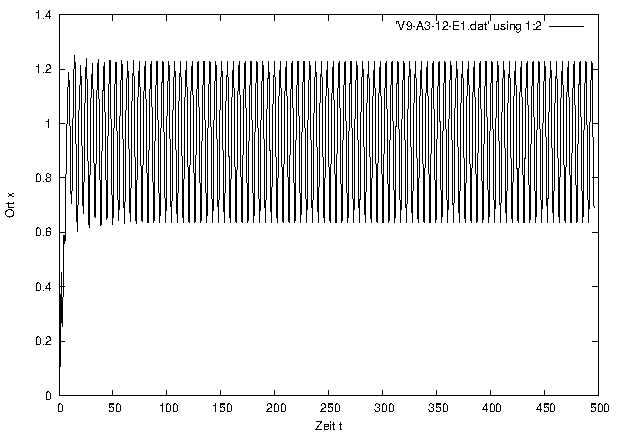
\includegraphics[width=10.411911321002231cm,height=7.288337924701561cm]{Vorlesung-9-1.pdf}}}
  \tmunfoldedio{GNUplot] }{set ylabel 'Ort x(t-tau)'; set xlabel 'Ort x(t)';
  plot 'V9-A3-12-E1.dat' using 2:3 with lines \# n =
  7}{\raisebox{0.0\height}{\includegraphics[width=10.411911321002231cm,height=7.288337924701561cm]{Vorlesung-9-2.pdf}}}
  \tminput{GNUplot] }{\ }
}

Nun Plot mit Ver{\"a}nderung des Paramters n.

Hier n = 7.75 dadurch Periodenverdoppelung

\tmsession{gnuplot}{default}{
  \tmunfoldedio{GNUplot] }{set ylabel 'Ort x(t-tau)'; set xlabel 'Ort x(t)';
  plot 'V9-A3-12-E2.dat' using 2:3 with lines \# n =
  7.75}{\raisebox{0.0\height}{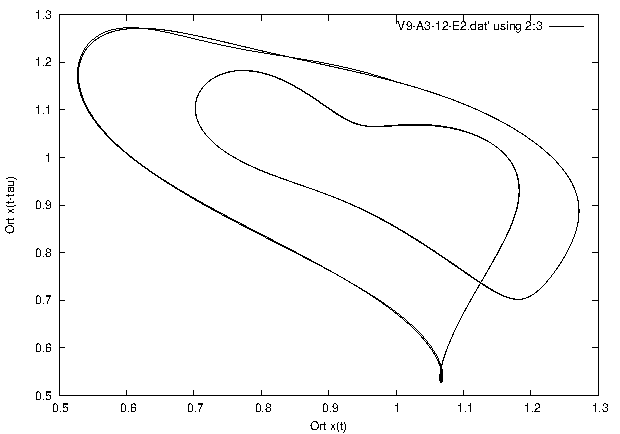
\includegraphics[width=10.411911321002231cm,height=7.288337924701561cm]{Vorlesung-9-3.pdf}}}
  \tmunfoldedio{GNUplot] }{set xlabel 'Zeit t'; set ylabel 'Ort x'; plot
  'V9-A3-12-E2.dat' using 1:2 with lines \# n =
  7.75}{\raisebox{0.0\height}{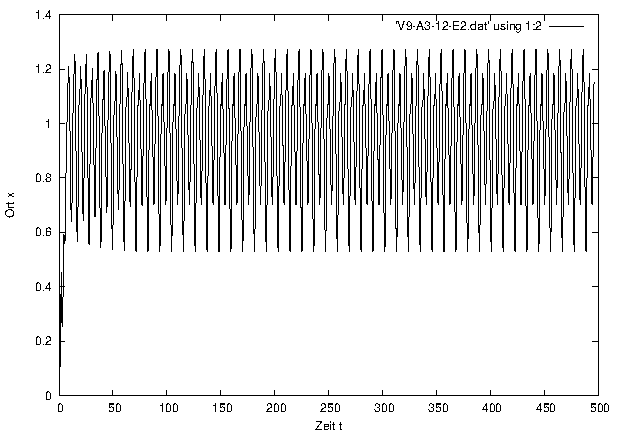
\includegraphics[width=10.411911321002231cm,height=7.288337924701561cm]{Vorlesung-9-4.pdf}}}
  \tminput{GNUplot] }{\ }
}

Hier n = 8.79 dadurch Periodenvervierfachung

\tmsession{gnuplot}{default}{
  \tmunfoldedio{GNUplot] }{set ylabel 'Ort x(t-tau)'; set xlabel 'Ort x(t)';
  plot 'V9-A3-12-E3.dat' using 2:3 with lines \# n =
  8.79}{\raisebox{0.0\height}{\includegraphics[width=10.411911321002231cm,height=7.288337924701561cm]{Vorlesung-9-5.pdf}}}
  \tmunfoldedio{GNUplot] }{set xlabel 'Zeit t'; set ylabel 'Ort x'; set xrange
  [0:200]; plot 'V9-A3-12-E3.dat' using 1:2 with lines \# n =
  8.97}{\raisebox{0.0\height}{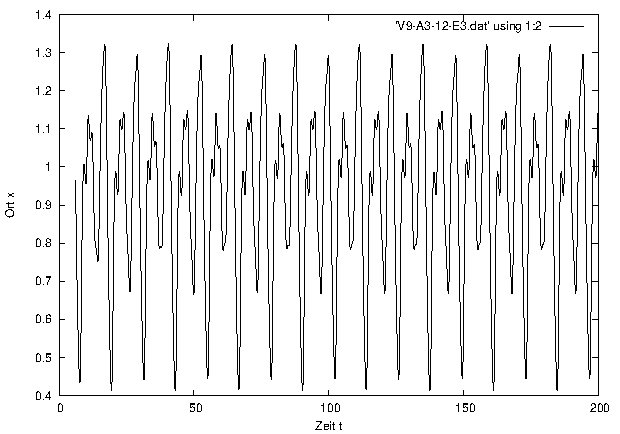
\includegraphics[width=10.411911321002231cm,height=7.288337924701561cm]{Vorlesung-9-6.pdf}}}
  \tminput{GNUplot] }{\ }
}

Hier n = 9.65 dadurch Chaos

\tmsession{gnuplot}{default}{
  \tmunfoldedio{GNUplot] }{set ylabel 'Ort x(t-tau)'; set xlabel 'Ort x(t)';
  plot 'V9-A3-12-E4.dat' using 2:3 with lines \# n =
  9.65}{\raisebox{0.0\height}{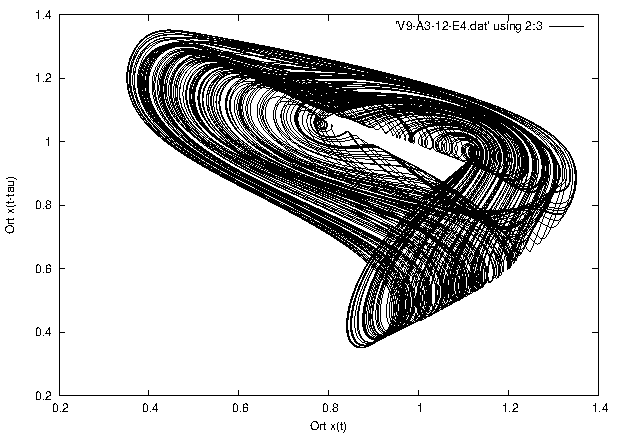
\includegraphics[width=10.411911321002231cm,height=7.288337924701561cm]{Vorlesung-9-7.pdf}}}
  \tmunfoldedio{GNUplot] }{set xlabel 'Zeit t'; set ylabel 'Ort x'; set xrange
  [400:1000]; plot 'V9-A3-12-E4.dat' using 1:2 with lines \# n =
  9.65}{\raisebox{0.0\height}{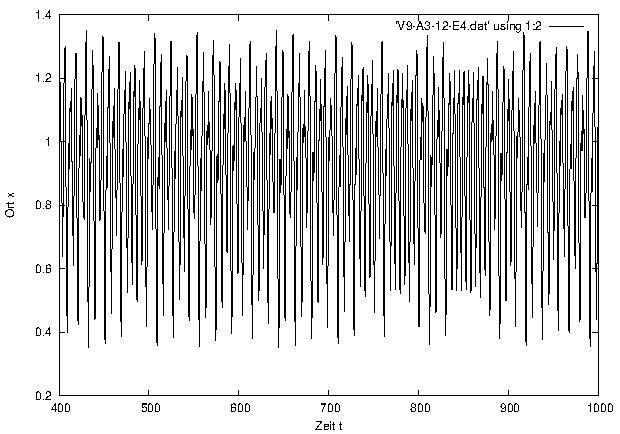
\includegraphics[width=10.411911321002231cm,height=7.288337924701561cm]{Vorlesung-9-8.pdf}}}
  \tminput{GNUplot] }{\ }
}

Hier n = 9.65 dadurch Chaos in 3D

\tmsession{gnuplot}{default}{
  \tmunfoldedio{GNUplot] }{set xlabel 'Ort x(t-tau)'; set ylabel 'Ort x(t)';
  set zlabel 'Ort x(t-2tau)'; splot 'V9-A3-12-E4.dat' using 2:3:4 with lines
  \# n =
  9.65}{\raisebox{0.0\height}{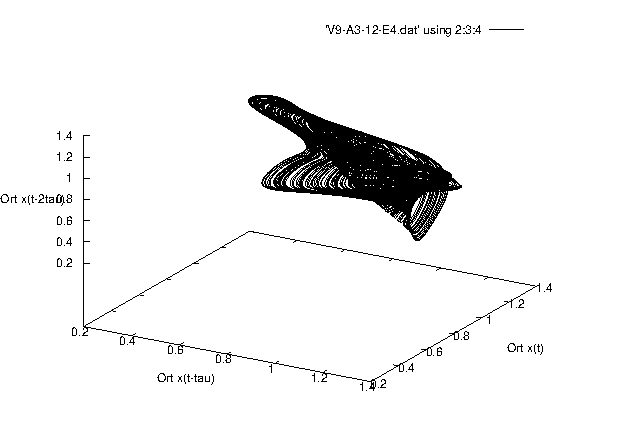
\includegraphics[width=10.411911321002231cm,height=7.288337924701561cm]{Vorlesung-9-9.pdf}}}
  \tminput{GNUplot] }{\ }
}

\end{document}
